\documentclass[aspectratio=1610, ]{beamer}%, handout
\usepackage{graphics}
\usepackage{pifont}
\usepackage{ulem}
\usepackage{xcolor}
\usepackage{modifycolor}
\usepackage{lipsum}
\usepackage{fontspec}
\usepackage{caption}
\renewcommand{\figurename}{FIGURE}
\captionsetup[figure]{labelfont={color=leftFootlineColor, scriptsize}, textfont={color=normalBlockColor, scriptsize}}
\usepackage{tabularx}
\newcolumntype{Y}{>{\centering\arraybackslash}X}
\usepackage{tikz}
\usepackage{standalone}
\usepackage{svg}
\usepackage{multicol}
\usepackage{catchfilebetweentags}
\usepackage{xifthen}
\usetikzlibrary{arrows}
\usetikzlibrary{backgrounds}
\setmonofont[
  Contextuals={Alternate}
]{FuraCode Nerd Font}
\setsansfont{Roboto Medium}
\usepackage{pgfpages}


\usepackage[cache=false,outputdir=build]{minted}
\definecolor{bg_code}{HTML}{282828}
\usemintedstyle{darcula}
\setminted{
      fontsize=\scriptsize, 
      linenos,
      numbersep=0pt,
      gobble=5,
      framesep=3mm} 
      \renewcommand{\theFancyVerbLine}{\texttt{{{\arabic{FancyVerbLine}}}}}
\usepackage{adjustbox}
\usepackage{environ}%
\usepackage{tikz}
\usetikzlibrary{patterns}
\usepackage[french]{babel}
\usepackage{beamerthemesideblue}


\setbeamerfont{note page}{size=\footnotesize}
\setbeamertemplate{note page}[custom]
\setbeamercolor{note page}{bg=backgroundColor, fg=white}

\newcommand{\insertlicense}{
\includegraphics[height=1cm]{img/by-sa.png}}
\title[]{La rétroingénierie appliquée à Android}
\subtitle{La traque aux traqueurs}
\author{Maxime Catrice}
\date{\today}
\titlegraphic{
\includegraphics[height=0.95cm]{logo.png}\bigbreak\insertlicense}

\setbeamertemplate{title page}[default][colsep=-4bp,rounded=true,shadow=false]
\setbeamercolor{background canvas}{bg=backgroundColor}
\setbeamertemplate{blocks}[rounded][shadow=false]
\beamertemplatenavigationsymbolsempty
\newcounter{acolumn}%  Number of current column
\newlength{\acolumnmaxheight}%   Maximum column height
%%%%%%%%%%%%%%%%%%%%%%%%%


\makeatletter

% `column` replacement to measure height
\newenvironment{@acolumn}[1]{%
    \stepcounter{acolumn}%
    \begin{lrbox}{\@tempboxa}%
    \begin{minipage}{#1}%
}{%
    \end{minipage}
    \end{lrbox}
    \@tempdimc=\dimexpr\ht\@tempboxa+\dp\@tempboxa\relax
    % Save height of this column:
    \expandafter\xdef\csname acolumn@height@\roman{acolumn}\endcsname{\the\@tempdimc}%
    % Save maximum height
    \ifdim\@tempdimc>\acolumnmaxheight
        \global\acolumnmaxheight=\@tempdimc
    \fi
}

% `column` wrapper which sets the height beforehand
\newenvironment{@@acolumn}[1]{%
    \stepcounter{acolumn}%
    % The \autoheight macro contains a \vspace macro with the maximum height minus the natural column height
    \edef\autoheight{\noexpand\vspace*{\dimexpr\acolumnmaxheight-\csname acolumn@height@\roman{acolumn}\endcsname\relax}}%
    % Call original `column`:
    \orig@column{#1}%
}{%
    \endorig@column
}

% Save orignal `column` environment away
\let\orig@column\column
\let\endorig@column\endcolumn

% `columns` variant with automatic height adjustment
\NewEnviron{acolumns}[1][]{%
    % Init vars:
    \setcounter{acolumn}{0}%
    \setlength{\acolumnmaxheight}{0pt}%
    \def\autoheight{\vspace*{0pt}}%
    % Set `column` environment to special measuring environment
    \let\column\@acolumn
    \let\endcolumn\end@acolumn
    \BODY% measure heights
    % Reset counter for second processing round
    \setcounter{acolumn}{0}%
    % Set `column` environment to wrapper
    \let\column\@@acolumn
    \let\endcolumn\end@@acolumn
    % Finally process columns now for real
    \begin{columns}[#1]%
        \BODY
    \end{columns}%
}
\makeatother
%%%%%%%%%%%%%%%%%%%%%%%%%

\NewEnviron{frameNoSB}{
\makeatletter
\setbeamertemplate{sidebar canvas left}{}
\setbeamertemplate{sidebar left}{}
\makeatother
\begin{frame}
    \BODY
%\tableofcontents
\end{frame}
}

\NewEnviron{frameTitle}{
\setbeamertemplate{frametitle}[default][center]
\makeatletter
\setbeamertemplate{headline}{\color{backgroundColor}45\newline 45\newline 45\newline 45\newline 45\newline 45\newline 45\newline 45\newline 45\newline 45}
\setbeamertemplate{sidebar canvas left}{}
\setbeamertemplate{sidebar left}{}



\makeatother
\begin{frame}
\begin{minipage}[c]{\linewidth-\beamerleftmargin+\beamerrightmargin}
\BODY
\end{minipage}
\end{frame}
}

\setbeamerfont{title}{series=\bfseries,parent=structure}
\setbeamerfont{subtitle}{size=\Large,series=,parent=structure}

\makeatletter
\newlength\beamerleftmargin
\setlength\beamerleftmargin{\Gm@lmargin}

\newlength\beamerrightmargin
\setlength\beamerrightmargin{\Gm@rmargin}
\makeatother

\newcommand{\nologo}{\setbeamertemplate{logo}{}}

\newcommand{\slidetitle}[1][]{
  \frametitle{\insertsection\ifthenelse{\equal{#1}{}}{}{: #1}}
}
\newcommand{\mono}[1]{
\texttt{#1}
}

\setbeameroption{show notes on second screen=top}
\begin{document}
\section{Élévation de privilèges}
  \begin{frame}
    \slidetitle[]
    \noindent
    \begin{columns}
      \begin{column}{0.7\linewidth}
        \note{\ExecuteMetaData[004-elepriv_notes.tex]{Elepriv}}
        \note{\onslide->{<\ExecuteMetaData[004-elepriv_notes.tex]{Interet}}}
        \begin{block}{Qu'est ce qu'une élévation de privilège?}<2->
          \onslide<3->{
          Obtension de permissions accordées à un utilisateur supérieures aux permissions qu'il possède
          }
        \end{block}
        \begin{block}{Intérêt:}<4->
          \begin{itemize}
            \item<5-> Android est un système qui restreint l'utilisateur
            \item<6-> Accéder aux fonctionnalités bloquées
            \item<7-> Modifier en profondeur le fonctionnement des applications
          \end{itemize}
        \end{block}
      \end{column}
      \begin{column}{0.25\linewidth}
        
\includegraphics[width=1\linewidth]{img/android_root.png}
      \end{column}
    \end{columns}
  \end{frame}

  \begin{frame}[t]
    \slidetitle[Root]
    \note{\ExecuteMetaData[004-elepriv_notes.tex]{Root}}
    \note{\ExecuteMetaData[004-elepriv_notes.tex]{RootPrincipe}}
    \note{\ExecuteMetaData[004-elepriv_notes.tex]{RootExemples}}
    \begin{block}{Qu'est ce que le root?}<2->
      \onslide<3->{
      Obtention de permissions avancées pour l'utilisateur (``droits super- utilisateurs''), permettant de contourner les limitations constructeurs
      }
    \end{block}
    \begin{columns} 
      \begin{column}{0.7\linewidth}
        \begin{overlayarea}{\linewidth}{0.5\textheight}
        \only<3-8|handout:1>{
        \begin{block}{Principe du root: \mono{/system}}<4->
          \begin{enumerate}
          \item<5-> Utilisation d'une vulnérabilité par un processus pour changer son uid à 0
          \item<6-> Remontage de la partition \mono{/system} en écriture
          \item<7-> Copie des binaires su, busybox
          \item<8-> Remontage de \mono{/system} en lecture seule
          \end{enumerate}
        \end{block}
        }
        \only<9-|handout:2>{
          \begin{block}{Exemples d'utilisation}
            \begin{itemize}
            \item<10-> Accéder aux partitions systèmes
            \item<11-> Ajouter un binaire BusyBox
            \item<12-> Sauvegarder l'état actuel d'une application
            \item<13-> Modifier les propriétés systèmes
            \end{itemize}
          \end{block}
        }
        \end{overlayarea}
      \end{column}
      \begin{column}{0.25\linewidth}
        \centering
        
\includegraphics[width=\linewidth]{img/superSU.png}
      \end{column}
    \end{columns}
  \end{frame}


  \begin{frame}[t]
    \slidetitle[Xposed]
    \note{\ExecuteMetaData[004-elepriv_notes.tex]{Xposed}}
    \note{\ExecuteMetaData[004-elepriv_notes.tex]{XposedUtilisation}}
    \begin{block}{Qu'est ce que le module Xposed?}<2->
      \onslide<3->{
      Framework permettant d'intercepter toutes méthodes d'une application, pour injecter du code suplémentaire
      }
    \end{block}
    \begin{columns} 
      \begin{column}{0.7\linewidth}
        \begin{block}{Exemple d'utilisation}<4->
          \begin{itemize}
          \item<5-> Lire les preferences 
          \item<6-> Désactiver la vérification des certificats SSL
          \item<7-> Modifier son IMEI
          \item<8-> Modifier sa position GPS
          \end{itemize}
        \end{block}
      \end{column}
      \begin{column}{0.25\linewidth}
        \centering
        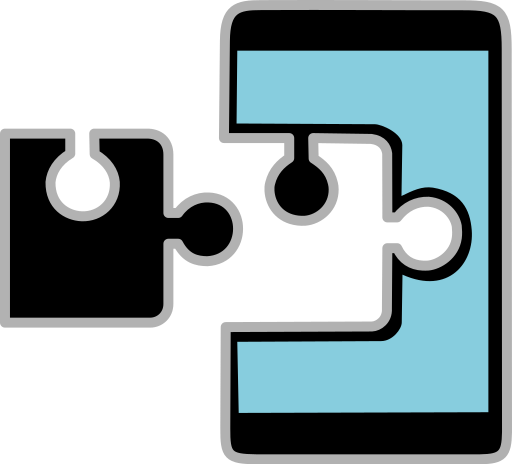
\includegraphics[width=0.9\linewidth]{img/xposed.png}
      \end{column}
    \end{columns}
  \end{frame}


  \begin{frame}[t]
    \slidetitle[Xposed]
    \pause
    \note{\ExecuteMetaData[004-elepriv_notes.tex]{BootAndroid}}
    \note{\onslide<7->{\ExecuteMetaData[004-elepriv_notes.tex]{Zygote}}}
    \note{\onslide<12->{\ExecuteMetaData[004-elepriv_notes.tex]{XposedFonctionnement}}}
    \begin{columns} 
      \begin{column}{0.4\linewidth}
        \vspace{-1.25cm}
        \centering
        \begin{figure}
          \documentclass[aspectratio=1610,]{beamer}%, handout
\usepackage{tikz}
\usepackage{graphics}
\usepackage{pifont}
\usepackage{ulem}
\usepackage{xcolor}
\usepackage{modifycolor}
\usepackage{lipsum}
\usepackage{fontspec}
\usepackage{caption}
\renewcommand{\figurename}{FIGURE}
\captionsetup[figure]{labelfont={color=leftFootlineColor, scriptsize}, textfont={color=normalBlockColor, scriptsize}}
\usepackage{tabularx}
\newcolumntype{Y}{>{\centering\arraybackslash}X}
\usepackage{tikz}
\usepackage{standalone}
\usepackage{svg}
\usepackage{multicol}
\usepackage{catchfilebetweentags}
\usepackage{xifthen}
\usetikzlibrary{arrows}
\usetikzlibrary{backgrounds}
\setmonofont[
  Contextuals={Alternate}
]{FuraCode Nerd Font}
\setsansfont{Roboto Medium}
\usepackage{pgfpages}


\usepackage[cache=false,outputdir=build]{minted}
\definecolor{bg_code}{HTML}{282828}
\usemintedstyle{darcula}
\setminted{
      fontsize=\scriptsize, 
      linenos,
      numbersep=0pt,
      gobble=5,
      framesep=3mm} 
      \renewcommand{\theFancyVerbLine}{\texttt{{{\arabic{FancyVerbLine}}}}}
\usepackage{adjustbox}
\usepackage{environ}%
\usepackage{tikz}
\usetikzlibrary{patterns}
\usepackage[french]{babel}
\usepackage{beamerthemesideblue}


\setbeamerfont{note page}{size=\footnotesize}
\setbeamertemplate{note page}[custom]
\setbeamercolor{note page}{bg=backgroundColor, fg=white}

\newcommand{\insertlicense}{
\includegraphics[height=1cm]{img/by-sa.png}}
\title[]{La rétroingénierie appliquée à Android}
\subtitle{La traque aux traqueurs}
\author{Maxime Catrice}
\date{\today}
\titlegraphic{
\includegraphics[height=0.95cm]{logo.png}\bigbreak\insertlicense}

\setbeamertemplate{title page}[default][colsep=-4bp,rounded=true,shadow=false]
\setbeamercolor{background canvas}{bg=backgroundColor}
\setbeamertemplate{blocks}[rounded][shadow=false]
\beamertemplatenavigationsymbolsempty
\newcounter{acolumn}%  Number of current column
\newlength{\acolumnmaxheight}%   Maximum column height
%%%%%%%%%%%%%%%%%%%%%%%%%


\makeatletter

% `column` replacement to measure height
\newenvironment{@acolumn}[1]{%
    \stepcounter{acolumn}%
    \begin{lrbox}{\@tempboxa}%
    \begin{minipage}{#1}%
}{%
    \end{minipage}
    \end{lrbox}
    \@tempdimc=\dimexpr\ht\@tempboxa+\dp\@tempboxa\relax
    % Save height of this column:
    \expandafter\xdef\csname acolumn@height@\roman{acolumn}\endcsname{\the\@tempdimc}%
    % Save maximum height
    \ifdim\@tempdimc>\acolumnmaxheight
        \global\acolumnmaxheight=\@tempdimc
    \fi
}

% `column` wrapper which sets the height beforehand
\newenvironment{@@acolumn}[1]{%
    \stepcounter{acolumn}%
    % The \autoheight macro contains a \vspace macro with the maximum height minus the natural column height
    \edef\autoheight{\noexpand\vspace*{\dimexpr\acolumnmaxheight-\csname acolumn@height@\roman{acolumn}\endcsname\relax}}%
    % Call original `column`:
    \orig@column{#1}%
}{%
    \endorig@column
}

% Save orignal `column` environment away
\let\orig@column\column
\let\endorig@column\endcolumn

% `columns` variant with automatic height adjustment
\NewEnviron{acolumns}[1][]{%
    % Init vars:
    \setcounter{acolumn}{0}%
    \setlength{\acolumnmaxheight}{0pt}%
    \def\autoheight{\vspace*{0pt}}%
    % Set `column` environment to special measuring environment
    \let\column\@acolumn
    \let\endcolumn\end@acolumn
    \BODY% measure heights
    % Reset counter for second processing round
    \setcounter{acolumn}{0}%
    % Set `column` environment to wrapper
    \let\column\@@acolumn
    \let\endcolumn\end@@acolumn
    % Finally process columns now for real
    \begin{columns}[#1]%
        \BODY
    \end{columns}%
}
\makeatother
%%%%%%%%%%%%%%%%%%%%%%%%%

\NewEnviron{frameNoSB}{
\makeatletter
\setbeamertemplate{sidebar canvas left}{}
\setbeamertemplate{sidebar left}{}
\makeatother
\begin{frame}
    \BODY
%\tableofcontents
\end{frame}
}

\NewEnviron{frameTitle}{
\setbeamertemplate{frametitle}[default][center]
\makeatletter
\setbeamertemplate{headline}{\color{backgroundColor}45\newline 45\newline 45\newline 45\newline 45\newline 45\newline 45\newline 45\newline 45\newline 45}
\setbeamertemplate{sidebar canvas left}{}
\setbeamertemplate{sidebar left}{}



\makeatother
\begin{frame}
\begin{minipage}[c]{\linewidth-\beamerleftmargin+\beamerrightmargin}
\BODY
\end{minipage}
\end{frame}
}

\setbeamerfont{title}{series=\bfseries,parent=structure}
\setbeamerfont{subtitle}{size=\Large,series=,parent=structure}

\makeatletter
\newlength\beamerleftmargin
\setlength\beamerleftmargin{\Gm@lmargin}

\newlength\beamerrightmargin
\setlength\beamerrightmargin{\Gm@rmargin}
\makeatother

\newcommand{\nologo}{\setbeamertemplate{logo}{}}

\newcommand{\slidetitle}[1][]{
  \frametitle{\insertsection\ifthenelse{\equal{#1}{}}{}{: #1}}
}
\newcommand{\mono}[1]{
\texttt{#1}
}

\definecolor{backgroundColor}{HTML}{2D2D2D}
\usetikzlibrary{arrows}
\usetikzlibrary{backgrounds}
\begin{document}
\begin{tikzpicture}[scale=0.45, every node/.style={scale=0.6},show background rectangle,
    background rectangle/.style={fill=backgroundColor},color=white,]
    \tikzstyle{myarrows}=[thick, line width=1.3mm,-open triangle 90,
    postaction={draw, line width=2.5mm, shorten >=3mm, -},
    postaction={draw, backgroundColor, shorten >= 0.4mm, -triangle 90, line width=1.05mm},
    postaction={draw, line width=2mm, backgroundColor, shorten >= 4mm, -}]
    \tikzstyle{myarrows_back}=[thick, line width=1.7mm,-open triangle 90,
    postaction={draw, line width=6.5mm, shorten >=4mm, -},
    postaction={draw, backgroundColor, shorten >= 1.3mm, -triangle 90, line width=1mm},
    postaction={draw, line width=5mm, backgroundColor, shorten >= 4mm, -}]
    
\draw [ultra thick, rounded corners=5] (0,0) rectangle node{
Kernel
} (3,-1.5);
\node[inner sep=0,minimum size=0] at (1.5,-1.55) (K) {}; % invisible node
\draw [ultra thick, rounded corners=5] (0,-3.5) rectangle node{
Init
} (3,-5);
\node[inner sep=0,minimum size=0] at (1.5,-3.5) (I0) {}; % invisible node
\node[inner sep=0,minimum size=0] at (-0.05,-4.25) (I1) {}; % invisible node
\node[inner sep=0,minimum size=0] at (3.05,-4.25) (I2) {}; % invisible node
\node[inner sep=0,minimum size=0] at (1.5,-5.05) (II) {}; % invisible node

\draw [ultra thick, rounded corners=5] (0,-3.5) rectangle node{
Init
} (3,-5);

\draw[myarrows] (K) to (I0);

\node[inner sep=0,minimum size=0] at (1.5,-3.5) (Z0) {}; % invisible node
\node[inner sep=0,minimum size=0] at (1.5,-8.55) (Z1) {}; % invisible node
\onslide<1-5|handout:1>{\draw [ultra thick, rounded corners=5] (0,-7) rectangle node{
Zygote
} (3,-8.5);}

\node[inner sep=0,minimum size=0] at (1.5,-7) (Z0) {}; % invisible node
\draw[myarrows] (II) to (Z0);


\draw [ultra thick, rounded corners=5] (-4,-7) rectangle node{
Demons
} (-1,-8.5);
\node[inner sep=0,minimum size=0] at (-2.5,-7) (D) {}; % invisible node
\draw[myarrows] (I1) -| (D);

\draw [ultra thick, rounded corners=5] (4,-7) rectangle node{
Runtime
} (7,-8.5);
\node[inner sep=0,minimum size=0] at (5.5,-7) (R) {}; % invisible node
\draw[myarrows] (I2) -| (R);

\node[inner sep=0,minimum size=0] at (1.5,-10.5) (VM0) {}; % invisible node
\node[inner sep=0,minimum size=0] at (1.5,-12) (VM1) {}; % invisible node
\draw [ultra thick, rounded corners=5] (0,-10.5) rectangle node{
VM
} (3,-12);
\draw[myarrows] (Z1) to (VM0);

\node[inner sep=0,minimum size=0] at (1.5,-15) (APP) {}; % invisible node
\draw [ultra thick, rounded corners=5] (0,-15) rectangle node{
Applications
} (3,-16.5);
\draw[myarrows] (VM1) to (APP);

\fill [backgroundColor] (0,-12.5) rectangle (3,-13.5);
\draw [ultra thick, rounded corners=5] (1.5,-13) node{
{\LARGE \textbullet\textbullet\textbullet}
} (3,-13.5);

\onslide<6-|handout:2>{\draw [ultra thick, rounded corners=5, red] (0,-7) rectangle node{
Zygote
} (3,-8.5);}
\end{tikzpicture}
\end{document}

          \vspace{-0.75cm}
          \caption{Initialisation d'Android}
        \end{figure}
      \end{column}
    
      \begin{column}{0.55\linewidth}
      \vspace{-1cm}%
        \centering
        \only<3-11|handout:1>{
          \begin{block}{Démarrage d'Android}<3-11>
            \begin{enumerate}
            \item <4-> Le kernel lance le processus init
            \item <5-> Init lance des demons, runtime
            % usb, adb, ril...
            \item <6-> Init lance Zygote
            \end{enumerate}
        \end{block}

        \begin{block}{Le processus Zygote:}<7-11>
          \begin{enumerate}
          \item <8-> Initialise une instance de la VM
          \item <9-> Pré-charge des classes
          \item <10-> Fork pour chaque application
          % usb, adb, ril...
          \item <11-> Partage une partie de sa mémoire avec ses fils
          \end{enumerate}
      \end{block}
        }
        \only<12-|handout:2>{
          \begin{block}{Fonctionnement}
            \begin{enumerate}
              \item <13-> Modification du processus init pour ajouter des librairies au classpath
              \item <14-> Ajout de librairies à Zygote pour détecter le lancement d'applications
              \item <15-> A chaque nouvelle aplication forké de Zygote, il est possible de modifier le code exécuté lar la VM
              \end{enumerate}
        \end{block}
        }
      \end{column}
    \end{columns}
  \end{frame}
\end{document}